\documentclass[UTF-8,twoside,cs4size]{ctexart}
\usepackage[dvipsnames]{xcolor}
\usepackage{amsmath}
\usepackage{amssymb}
\usepackage{geometry}
\usepackage{setspace}
\usepackage{xeCJK}
\usepackage{ulem}
\usepackage{pstricks}
\usepackage{pstricks-add}
\usepackage{bm}
\usepackage{mathtools}
\usepackage{breqn}
\usepackage{mathrsfs}
\usepackage{esint}
\usepackage{textcomp}
\usepackage{upgreek}
\usepackage{pifont}
\usepackage{tikz}
\usepackage{circuitikz}
\usepackage{caption}
\usepackage{tabularx}
\usepackage{array}
\newcolumntype{Y}{>{\centering\arraybackslash}X}
\usepackage{pgfplots}
\usepackage{multirow}
\usepackage{pgfplotstable}
\usepackage{mhchem}
\usepackage{physics} % Add this package for \dt and \dif commands
\newcommand{\dif}{\mathrm{d}}
\usepackage{cases}
\usepackage{subfigure}
\usepackage{enumerate}
\usepackage{minipage-marginpar}
\usepackage{diagbox}
\usepackage{graphicx}


\graphicspath{{./figure/}}

\setCJKfamilyfont{zhsong}[AutoFakeBold = {5.6}]{STSong}
\newcommand*{\song}{\CJKfamily{fangsong}}

\geometry{a4paper,left=2cm,right=2cm,top=0.75cm,bottom=2.54cm}

\newcommand{\experiName}{弦上驻波及介质中声速测量}%实验名称
\newcommand{\supervisor}{王智茂}%指导教师
\newcommand{\name}{孙奕飞}
\newcommand{\studentNum}{2023k8009925001}
\newcommand{\class}{2}%班级
\newcommand{\group}{06}%组
\newcommand{\seat}{01}%座位号
\newcommand{\dateYear}{2024}
\newcommand{\dateMonth}{12}%月
\newcommand{\dateDay}{10}%日
\newcommand{\room}{教721}%地点
\newcommand{\others}{$\square$}

\ctexset{
    section={
        format+=\raggedright\song\large
    },
    subsection={
        name={\quad,.}
    },
    subsubsection={
        name={\qquad,.}
    }
}

\begin{document}
\noindent

\begin{center}

    \textbf{\song \zihao{-2} \ziju{0.5}《基础物理实验》实验报告}
    
\end{center}


\begin{center}
    \kaishu \zihao{5}
    \noindent \emph{实验名称}\underline{\makebox[28em][c]{\experiName}}
    \emph{指导教师}\underline{\makebox[9em][c]{\supervisor}}\\
    \emph{姓名}\underline{\makebox[6em][c]{\name}} 
    \emph{学号}\underline{\makebox[14em][c]{\studentNum}}
    \emph{分班分组及座号} \underline{\makebox[5em][c]{\class \ -\ \group \ -\ \seat }\emph{号}} \\
    \emph{实验日期} \underline{\makebox[3em][c]{\dateYear}} \emph{年}
    \underline{\makebox[2em][c]{\dateMonth}}\emph{月}
    \underline{\makebox[2em][c]{\dateDay}}\emph{日}
    \emph{实验地点}\underline{{\makebox[4em][c]\room}}
    \emph{调课/补课} \underline{\makebox[3em][c]{否}}
    \emph{成绩评定} \underline{\hspace{8em}}
    {\noindent}
    \rule[5pt]{17.7cm}{0.2em}
\end{center}

\begin{center}
    \Large\bfseries 第一部分\quad 弦上驻波实验
\end{center}
\section{实验目的}
\begin{enumerate}
    \item 理解驻波的概念,观察弦线上的驻波现象,并掌握弦线形成共振以及稳定驻波的条件;
    \item 测量弦线上横波的传播速度;
    \item 通过实验研究弦线在受迫振动时的共振频率 $f$ 与半波长数目 $n$、弦线有效长度 $L$、张力 $T$ 及弦密度之间的关系;
    \item 利用数学方法对实验数据进行处理,总结出共振频率与张力以及线密度之间的关系,并得出结论。
\end{enumerate}

\section{实验器材}
本实验的主要装置包括弦音计、信号发生器以及双踪示波器。此外,还配备了天平等测量工具。

\begin{enumerate}
    \item 弦音计由吉他弦、固定弦线的支架和基座、琴码、砝码支架、驱动线圈、探测线圈以及砝码等组成。其中,驱动线圈和探测线圈是装置中的关键部分。驱动线圈通过信号发生器提供一定频率的功率信号,产生交变磁力以驱动金属弦线产生振动;而探测线圈负责将弦线的振动信号转化为电信号,并通过示波器对其进行观测。

    \begin{figure}[!h]
        \centering
        \begin{tikzpicture}
            \filldraw[black,fill opacity=0.5] (0,1)--(0.7,1)--(0.9,0.8)--(1.1,0.8)--(1.3,1)--(1.7,1)--(1.9,0.8)--(2.1,0.8)--(2.3,1)--(2.7,1)--(2.9,0.8)--(3.1,0.8)--(3.3,1)--(3.7,1)--(3.9,0.8)--(4.1,0.8)--(4.3,1)--(4.7,1)--(4.9,0.8)--(5.1,0.8)--(5.3,1)--(6,1)--(6,0.5)--(0,0.5)--(0,1)--cycle;
            \draw[dashed] (1,1.5)--(1,-0.5);
            \draw[dashed] (2,2)--(2,-0.5);
            \draw[dashed] (3,2.5)--(3,-0.5);
            \draw[dashed] (4,3)--(4,-0.5);
            \draw[dashed] (5,3.5)--(5,-0.5);
            \draw[dashed] (0.7,-1) rectangle (1.3,-0.5);
            \draw[dashed] (1.7,-1) rectangle (2.3,-0.5);
            \draw[dashed] (2.7,-1) rectangle (3.3,-0.5);
            \draw[dashed] (3.7,-1) rectangle (4.3,-0.5);
            \draw[dashed] (4.7,-1) rectangle (5.3,-0.5);
            \node[below left] at(1,0.5) {1};
            \node[below left] at(2,0.5) {2};
            \node[below left] at(3,0.5) {3};
            \node[below left] at(4,0.5) {4};
            \node[below left] at(5,0.5) {5};
            \draw[->] (1,1.5)--(1.6,1.5) node[right]{$1mg$};
            \draw[->] (2,2)--(3.2,2) node[right]{$2mg$};
            \draw[->] (3,2.5)--(4.8,2.5) node[right]{$3mg$};
            \draw[->] (4,3)--(6.4,3) node[right]{$4mg$};
            \draw[->] (5,3.5)--(8,3.5) node[right]{$5mg$};
            \draw (-4,-1) rectangle (0,3);
            \node at(-2,1) {弦音计};
        \end{tikzpicture}
        \caption{弦音计中不同槽位的砝码对弦线的拉力示意图}
    \end{figure}
    
    \item 信号发生器采用低频功率信号发生器,其提供的输出信号频率范围可调,从 $10\,\mathrm{Hz}$ 覆盖至 $1\,\mathrm{kHz}$,用于向驱动线圈传输此范围内的正弦信号以产生振动。
    
    \item 双踪示波器的主要功能是用于检测信号源的波形,并实时显示探测线圈捕获的弦线振动波形,从而对弦线的振动现象进行直接观察。
\end{enumerate}

\section{实验原理}
将弦线两端固定,并在其一端附近使弦线做振幅固定的连续简谐振动。由此,一个由横波组成的波列将从该端向另一端传播。当前进波到达另一端时,会发生反射并返回原点;随后通过原点后再次反射,这样的过程不断重复。在弦线中,前进波和多次反射波同时存在。如果弦线长度和波长之间满足某种特定关系,使得前进波与所有反射波的相位相同,则弦线中各点会以固定振幅进行简谐振动。在驻波的形态下,某些点的振幅达到最大,称为波腹,而某些点振幅始终为零,称为波节。

\begin{figure}[!h]
    \centering
    \begin{tikzpicture}
        \draw [domain=0:4*pi,samples=1000,thick] plot (\x,{sin(2*\x r)});
        \draw [domain=0:4*pi,samples=1000,thick,dashed] plot (\x,{-sin(2*\x r)});
        \draw [->] (pi,-2.5)node[below]{波节}--(pi,-0.5);
        \draw [->] (2.75*pi,-2.5)node[below]{波腹}--(2.75*pi,-1.2);
        \draw [ultra thick] (0,-1.2)--(0,1.2);
        \draw [ultra thick] (4*pi,-1.2)--(4*pi,1.2);
    \end{tikzpicture}
    \caption{驻波现象示意图}
\end{figure}

在弦线驻波中,相邻的两个波腹或波节之间的距离 $D$ 为波长 $\lambda$ 的一半,即 $D = \frac{\lambda}{2}$,这一长度被称为半波长。由于弦线两端始终保持固定状态,两端必为波节。因此,弦线的总长度必须是半波长的整数倍。若弦线长度记为 $L$,则满足以下关系:
\[
L = nD = \frac{n\lambda}{2}, \qquad n = 1, 2, 3, \cdots
\]

假设弦线的振动频率为 $f$,横波在弦线上的传播速度为 $v$,则波速与波长 $\lambda$ 和频率 $f$ 的关系为 $v = f\lambda$。根据波动理论,如果拉紧弦线的张力为 $T$,而弦线的线密度为 $\mu$,在弦线上某一点的传播方向坐标为 $x$,振动位移为 $y$,则横波的传播满足以下波动方程:
\[
\frac{\partial^2 y}{\partial t^2} = \frac{T}{\mu} \frac{\partial^2 y}{\partial x^2}, \qquad \frac{\partial^2 y}{\partial t^2} = v^2 \frac{\partial^2 y}{\partial x^2}
\]
由此可得,横波在弦线中的传播速度满足关系:
\[
v = \sqrt{\frac{T}{\mu}}
\]

通过将上述关系与 $v=f\lambda$ 结合,可以比较理论预测值与实验测量值之间的差异,并分析可能的原因。

此外,振动频率 $f$ 与张力 $T$ 和线密度 $\mu$ 的关系可表示为:
\[
f = \frac{1}{\lambda} \sqrt{\frac{T}{\mu}}
\]
对上述关系的两边取对数,得:
\[
\ln f = \frac{1}{2} \ln T - \frac{1}{2} \ln \mu - \ln \lambda
\]

\section{实验内容}
\begin{enumerate}
    \item 熟悉实验所需仪器,并对其进行正确的调节;
    
    \item 测量实验中所用弦线的线密度。具体方法是,利用天平测出弦线的质量 $m$,并通过尺子测量弦线的长度 $L$。注意,应采用与实验用弦线直径相同的吉他弦样品,并取其中段长度约为 70-80\,cm,而不是直接从弦音计上拆下弦线进行测量。根据质量和长度的测量结果,弦线的线密度可通过以下公式计算:
    \[
    \mu = \frac{m}{L}
    \]
    
    \item 在弦线上观察驻波现象。在实验时,固定弦线的张力 $T$ 和有效长度 $L$,然后调整信号发生器的输出频率,从而在弦线上形成有 $n\;(n=1,2,3,\cdots)$ 个波腹的稳定驻波,观察波的形态。
    
    \item 测量弦线上横波的传播速度,具体采用以下两种方法进行比较:
    \begin{enumerate}
        \item 方法一:测量弦线的张力 $T$ 和线密度 $\mu$,根据公式 $v=\sqrt{\frac{T}{\mu}}$ ,计算横波的传播速度。
        \item 方法二:首先测量共振频率 $f$ 和波的有效长度 $L$,再通过公式 $\lambda = \frac{2L}{n}$ 计算波长 $\lambda$,然后利用公式 $v = \lambda f$ 得到波速。最后对两种方法得到的结果进行对比。
    \end{enumerate}
    
    \item 当弦线处于受迫振动中时,固定弦线的线密度与张力,并取基频(即 $n=1$),研究共振频率 $f$ 与弦线有效长度 $L$ 的关系,并记录实验数据。
    
    \item 固定弦线的线密度与有效长度,同样取基频(即 $n=1$),研究弦线共振频率 $f$ 与张力 $T$ 之间的关系,实验过程中记录相关数据。

    \item 将弦线的张力 $T$ 与有效长度 $L$ 固定下来,依旧保持基频(即 $n=1$),研究共振频率 $f$ 与弦线线密度 $\mu$ 的关系,并记录实验数据用于后续分析。
\end{enumerate}

\section{实验结果与数据处理}
\subsection{线密度测试}
\begin{table}[!h]
    \centering
    \renewcommand\arraystretch{1.5}
    \caption{线密度测试}
    \begin{tabularx}{\textwidth}{|c|Y|Y|Y|Y|}
        \hline
        \textbf{弦号}&\textbf{质量}(g)&\textbf{长度}(mm)&\textbf{直径}(mm)&\textbf{线密度}(kg/m)\\
        \hline
        1&0.403&70.50&0.970&$5.72\times 10^{-3}$\\
        \hline
    \end{tabularx}
\end{table}

\subsection{波速的测试}
将琴码分别放置在 150\,mm 和 650\,mm 位置时,弦线的有效长度为 $L=500\,\mathrm{mm}$。在此条件下,不同频率 $f_n\,(n=1,2,3)$ 对应的波长 $\lambda$ 可由公式 $\lambda = \frac{2L}{n}$ 计算得到。因此,对应的波速公式分别为:$v_1 = 2Lf_1$,$v_2 = Lf_2$,以及 $v_3 = \frac{2Lf_3}{3}$。实验过程中通过测量频率求得波速的具体数据如表所示:

\begin{table}[!h]
    \centering
    \renewcommand\arraystretch{1.5}
    \caption{利用 $v = \lambda f$ 测量波速}
    \begin{tabularx}{\textwidth}{|c|Y|Y|Y|Y|Y|Y|Y|}
        \hline
        \textbf{砝码位置}$k$ & $f_1\,(\mathrm{Hz})$ & $v_1\,(\mathrm{m/s})$ & $f_2\,(\mathrm{Hz})$ & $v_2\,(\mathrm{m/s})$ & $f_3\,(\mathrm{Hz})$ & $v_3\,(\mathrm{m/s})$ & $\bar{v}\,(\mathrm{m/s})$ \\
        \hline
        2 & 30.75 & 30.75 & 61.49 & 30.75 & 92.72 & 30.91 & 30.80 \\
        \hline
        3 & 39.08 & 39.08 & 77.35 & 38.68 & 116.23 & 38.74 & 38.83 \\
        \hline
        4 & 44.08 & 44.08 & 88.21 & 44.105 & 132.49 & 44.16 & 44.12 \\
        \hline
    \end{tabularx}
\end{table}

在实验中,弦线的右端受到大小为 $kmg\,(k=2,3,4)$ 的拉力,因此弦线的张力可表达为 $T = \frac{1}{2}kmg$。实验测量得到砝码的质量为 $m=506.93\,\mathrm{g}$。利用公式 $v = \sqrt{\frac{T}{\mu}}$,可以计算出波速,并将其与由 $v = \lambda f$ 计算得出的平均波速 $\bar{v}$ 进行比较。相关计算数据及相对误差见下表:

\begin{table}[!h]
    \centering
    \renewcommand\arraystretch{1.5}
    \caption{利用 $v = \sqrt{\frac{T}{\mu}}$ 测量波速}
    \begin{tabularx}{\textwidth}{|c|Y|Y|Y|Y|}
        \hline
        \textbf{砝码位置}$k$ & $T\,(\mathrm{N})$ & $v\,(\mathrm{m/s})$ & $\bar{v}\,(\mathrm{m/s})$ & \textbf{相对误差}\,\% \\
        \hline
        2 & 4.968 & 29.47 & 30.80 & 4.318 \\
        \hline
        3 & 7.452 & 36.10 & 38.83 & 7.030 \\
        \hline
        4 & 9.936 & 41.67 & 44.16 & 5.638 \\
        \hline
    \end{tabularx}
\end{table}

由上述结果可以看出,采用两种方法测得的波速数值在允许的误差范围内基本一致,但k=3组实验数据产生了较大误差,猜测误差主要来自于共振频率测量的不准确。
\begin{figure}[!h]
    \centering
    \includegraphics*[scale=0.08]{fig1.jpg}
    \caption{实验中观察到的波节}
\end{figure}

\subsection{频率与有效长度的关系}
将砝码勾在第2格,改变有效长度,测量基频$ f_1 $,数据实验数据如下:
	\begin{table}[!h]
		\centering
		\renewcommand\arraystretch{1.5}
		\caption{不同有效长度下的基频}
		\begin{tabularx}{\textwidth}{|c|Y|Y|Y|Y|Y|}
			\hline
			$ L\,(\mathrm{m}) $&0.640&0.480&0.320&0.240&0.160\\
			\hline
			$ f_1\,(\mathrm{Hz}) $&23.80&32.03&48.29&65.01&99.88\\
			\hline
		\end{tabularx}
	\end{table}

\subsection{频率与张力的关系}
为了进一步研究拉力对基频的影响,将琴码分别放置在 200\,mm 和 600\,mm 位置,固定弦线的有效长度为 $L=400\,\mathrm{mm}$。实验中将砝码依次放置在 1-5 格处,以形成不同的拉力 $T$,同时测量各拉力情况下弦线的基频 $f_1$,并记录对应的实验数据。实验测量结果如下表所示:

\begin{table}[!h]
    \centering
    \renewcommand\arraystretch{1.5}
    \caption{频率和张力的关系}
    \begin{tabularx}{\textwidth}{|c|Y|Y|Y|Y|Y|}
        \hline
        \textbf{砝码位置} & \textbf{1} & \textbf{2} & \textbf{3} & \textbf{4} & \textbf{5} \\
        \hline
        $T\,(\mathrm{N})$ & 2.484 & 4.968 & 7.452 & 9.936 & 12.420 \\
        \hline
        $\ln T$ & 0.910 & 1.603 & 2.008 & 2.296 & 2.519 \\
        \hline
        $f_1\,(\mathrm{Hz})$ & 28.78 & 40.92 & 48.68 & 56.11 & 62.03 \\
        \hline
        $\ln f_1$ & 3.360 & 3.712 & 3.885 & 4.027 &  4.128 \\
        \hline
    \end{tabularx}
\end{table}
根据上表绘制得到下面的
$lnf - lnT$曲线,并利用sciPy库进行线性拟合,得到斜率为$k = 0.475\approx\frac12 $可知$ \ln f_1=\frac 12\ln T+C $(此时$ C $为常数),即$ f_1\propto\sqrt{T} $.
与理论基本相符。
\begin{figure}[!h]
    \centering
    \includegraphics*[scale=0.63]{output1.png}
    \caption{$lnf_1 - lnT$拟合直线图}
\end{figure}
\newpage

\subsection{频率与线密度的关系}
在实验中,将琴码分别放置于 200\,mm 和 600\,mm 位置,固定弦线的有效长度为 $L=400\,\mathrm{mm}$。实验通过改变琴弦的粗细(即线密度 $\mu$ 的不同),在砝码固定于第 2 格时,测量了不同琴弦的基频 $f_1$。实验记录了琴弦直径、线密度 $\mu$ 以及相关的对数值 $\ln \mu$ 和 $\ln f_1$.
汇总自己与本组其他同学的数据,得到如下表格:

\begin{table}[!h]
    \centering
    \renewcommand\arraystretch{1.5}
    \caption{不同线密度琴弦的基频}
    \begin{tabularx}{\textwidth}{|Y|Y|Y|Y|Y|Y|Y|Y|Y|}
        \hline
        \textbf{弦号} & 1 & 2 & 3 & 4 & 6 & 7 & 8 & 12 \\
        \hline
        \textbf{直径} (mm) & 0.970 & 0.850 & 1.005 & 0.860 & 0.882 & 0.815 & 0.396 & 1.070 \\
        \hline
        \textbf{线密度} $\mu$ (kg/m) & $5.72 \times 10^{-3}$ & $3.36 \times 10^{-3}$ & $5.18 \times 10^{-3}$ & $3.47 \times 10^{-3}$ & $3.70 \times 10^{-3}$ & $3.47 \times 10^{-3}$ & $1.07 \times 10^{-3}$ & $5.77 \times 10^{-3}$ \\
        \hline
        \textbf{基频} $f_1$ (Hz) & 40.92 & 51.18 & 39.83 & 35.20 & 50.01 & 48.16 & 88.50 & 44.08 \\
        \hline
        $\ln \mu$ & $-5.164$ & $-5.696$ & $-5.263$ & $-5.664$ & $-5.599$ & $-5.664$ & $-6.840$ & $-5.155$ \\
        \hline
        $\ln f_1$ & 3.712 & 3.935 & 3.685 & 3.561 & 3.912 & 3.875 & 4.483 & 3.786 \\
        \hline
    \end{tabularx}
\end{table}
由上表数据绘制得到如下拟合图样:
\begin{figure}[!h]
    \centering
    \includegraphics*[scale=0.63]{output2.png}
    \caption{$lnf_1 - ln\mu$拟合直线图}
\end{figure}
观察图线发现4号琴弦同学的数据点明显偏离拟合直线,猜测可能是由于实验操作不当导致的数据误差,将该点作为坏点剔除后重新绘制图线,得到如下图样:
\newpage
\begin{figure}[!h]
    \centering
    \includegraphics*[scale=0.63]{output3.png}
    \caption{$lnf_1 - ln\mu$拟合直线图(剔除坏点后)}
\end{figure}
由拟合直线斜率$ k=-0.453$,在实验误差允许范围内可视为$k \approx -\frac{1}{2}$,由此可知$ \ln f_1=-\frac12\ln\mu+C $(此时$ C $为常数),即$ f_1\propto\frac{1}{\sqrt \mu} $。
实验数据与理论存在的误差可能原因在于收集到的不同同学的数据均存在误差,经过叠加后使得实验数据出现较大偏离。同时,大部分数据点的$ln \mu$均集中在-5.70和-5.20附近,缺乏较为均匀的数据点,使得拟合直线的斜率较难准确反映实验数据的真实情况。

\section{实验总结与心得体会}
\subsection{讲义思考题}
1. 调节振动源上的振动频率和振幅大小后会对弦线振动产生怎样的影响?

{\kaishu 弦线的振动是由振动源的驱动引起的。当调节振动源频率时,会改变弦线上前进波与反射波之间的干涉情况。在特定条件下,弦线可能形成驻波现象。而调节振动源的振幅,只会影响弦线上各点的振动振幅大小,却不会对是否产生驻波现象造成影响。}


2. 如何确定弦线上的波节点位置?

{\kaishu 如果进行粗略观测,可以通过肉眼直接识别弦线上振幅几乎为零的区域,这些位置即为波节点位置。}

{\kaishu 若需要更精确地定位波节点,则可以通过调节接收器的位置来完成。移动接收器的过程中,观察示波器上接收到的波形。当波形振幅处于最小值的位置时,即可确定为波节点所在。}

3. 在弦线上出现驻波的条件是什么?为什么在实验中需要将弦线的振动调节到驻波最稳定、最显著的状态?

{\kaishu 根据实验原理可知,驻波出现的条件为 $n\lambda = 2L\;(n=1,2,3,\cdots)$,即弦线的有效长度必须是半波长的正整数倍。}

{\kaishu 在实验中,将弦线的振动调节到驻波最稳定、最显著的状态,是为了使弦线接近满足驻波形成的条件,从而保证前进波与反射波在弦线上各点之间发生具有稳定相位差的干涉。这一状态能够确保测量的基频数据更加精确,进而提高实验结果的准确性。}

4. 在弹奏弦线乐器时,发出的声音音调与弦线的长度、粗细、松紧程度有何关系?为什么?

{\kaishu 在弹奏弦线乐器的过程中,弦线的长度越短、直径越小、拉紧程度越高,其发出的音调会越高。}

{\kaishu 发出声音的音调与弦线振动的频率 $f$ 直接相关。根据实验中得到的原理公式 $\ln f = \frac{1}{2}\ln T - \frac{1}{2}\ln \mu - \ln \lambda$ 可知,振动频率的表达式为 $ f \propto \frac{1}{L},~f \propto \frac{1}{\sqrt{\mu}},~f \propto \sqrt{T} $。因此,振动频率 $f$ 与弦线长度成反比,与弦线的线密度(粗细)成反比,与弦线的张力(松紧程度)成正比,从而弦线的长度、粗细及松紧程度共同决定了声音的音调。}

5. 若样品弦线与实验装置上的弦线直径略有差异,应如何判断是否需要修正?如何进行修正?

{\kaishu 若样品弦线直径与装置上弦线的直径存在细微差别,则需要对实验测得的线密度进行修正。对于同种材料,由于密度 $\rho$ 是恒定的,因此直径 $d_1$ 和 $d_2$ 不同的两根弦线,其线密度 $\mu_1$ 和 $\mu_2$ 具有以下关系:假设取相同长度 $l$,则有:}
\[
\frac{\rho \pi d_1^2 l / 4}{\rho \pi d_2^2 l / 4} = \frac{\mu_1 l}{\mu_2 l} \,\Longrightarrow\, \frac{d_1^2}{d_2^2} = \frac{\mu_1}{\mu_2}
\]
{\kaishu 可以看出,弦线的线密度 $\mu$ 与直径 $d$ 的平方成正比,即 $\mu \propto d^2$。}

{\kaishu 因此,修正方法如下:首先测量样品弦线的相关参数,并记录样品弦线直径 $d_2$;然后测量装置上弦线的直径 $d_1$,计算修正系数 $k = \frac{d_1}{d_2}$。接着,根据样品弦线的线密度 $\mu$,计算修正后的装置弦线的线密度 $\mu'$,修正公式为:}
\[
\mu' = k^2 \mu = \left(\frac{d_1}{d_2}\right)^2 \mu
\]
{\kaishu 由此得到的 $\mu'$ 即为后续数据处理中需要使用的装置弦线的实际线密度。}

6. 对于某一共振频率,在增大或减小频率的调节过程中,为什么振幅最大的频率位置会有所不同?

{\kaishu 驻波现象可以在一定范围内相近的频率下被观察到,但波列本身并非完全稳定。在实验过程中,由于频率不断增大或减小的调节,可能引入人为误差或回调误差,从而影响振幅最大的频率位置。此外,实验条件(如弦线张力、小幅扰动等)可能引起微小变化,这些因素共同导致振幅最大的频率位置有所不同。}


\subsection{实验心得}
实验整体难度不大,在对横波的描述、波的干涉、驻波现象等知识有一定了解后,对于实验的理解体会也将不会构成难题。
但在实验操作上仍然有许多需要注意的地方,尤其是在调节振动源频率寻找驻波频率时,若操作不当会引起较大误差。
实验中,寻找驻波频率主要依靠观察示波器上的波形振幅实现的。然而,示波器本身无法直接给出振幅最大点位时的频率,需要通过肉眼观测寻找,因而存在较大误差。
同时,在绘制频率与线密度的关系图线时,需要注意剔除掉与图线整体趋势偏差明显的坏点,以保证拟合直线的准确性和实验数据整体的可靠性。


\begin{center}
    \Large\bfseries 第二部分\quad 测定介质中的声速
\end{center}
\setcounter{section}{0}
\section{实验目的}

\begin{enumerate}
    \item 掌握通过驻波法和相位法两种不同方法测量波长的实验技术;
    \item 计算超声波在空气和水中传播的速度;
    \item 学习声速测量仪、超声转换器等新型实验仪器的使用方法。
\end{enumerate}

\section{实验器材}
SW-2型声速测量仪,超声换能器,信号发生器,示波器,水槽,导线若干。

\section{实验原理}
\subsection{利用驻波法测量声速}

利用信号发生器输出的正弦电压信号,通过超声发射换能器将电信号转换为超声波发射出去,再由接收换能器将超声波通过声电转换生成电压信号,并将其送入示波器进行观察。

当接收换能器的接收面与发射换能器的发生面严格平行时,入射波会在接收面上发生垂直反射,入射波与反射波相互干涉,从而形成驻波。此时,如果两换能器之间的距离恰好是超声波波长的一半的整数倍,则可以在接收换能器端面观测到声压变化来判断驻波的形成。

通过转动鼓轮改变两换能器之间的距离,驻波将在一系列特定位置出现稳定状态。记录接收到最大电压值时标尺上的读数,相邻两次最大电压对应的距离之差即为半波长。

已知超声波的频率 $f$,并利用上述方法测得波长 $\lambda$,可以通过公式 $v = \lambda f$ 计算超声波的传播速度 $v$。

\subsection{利用相位法测量声速}

通过将发射波和接收波同时输入示波器,并设置为 X-Y 模式显示,能够观察两波的频率相同但相位不同的关系。当接收点与发射点的距离变化正好等于波长的整数倍时,相位差为 $2\pi$ 的整数倍,表现在实验中即为相位差等效为 $2\pi$。

在实验过程中,通过改变发射器与接收器之间的距离,观察示波器上的李萨如图形变化以判断相位变化。当相位变化 $\pi$ 时,相应距离的改变量即为波长的一半(半波长)。已知发射波的频率 $f$,根据公式 $v = \lambda f$ 就可以计算出声速。

当相位发生改变时,可通过李萨如图形直观地观察到其变化。部分典型的李萨如图形如下:
\begin{figure}[!h]
    \centering
    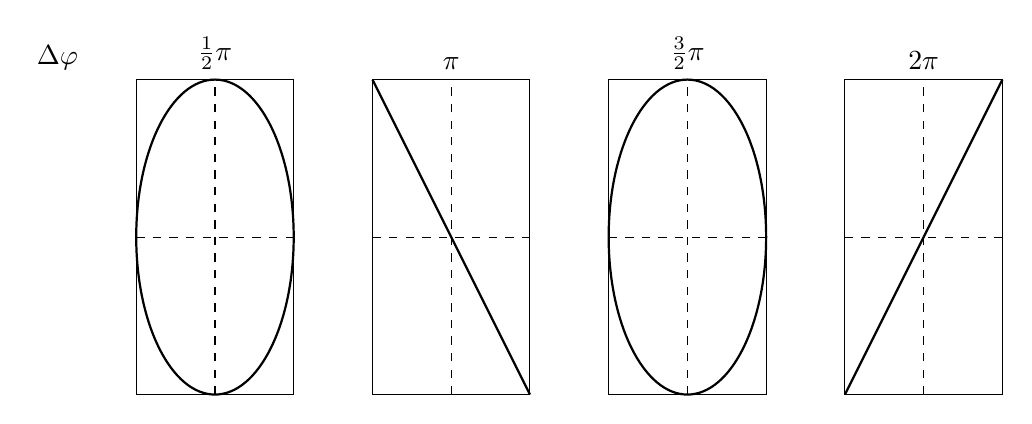
\begin{tikzpicture}
        % 图形1
        \draw [thick] (0,0) ellipse (1 and 2);
        \draw (-1,-2) rectangle (1,2);
        \draw [dashed] (-1,0)--(1,0);
        \draw [dashed] (0,-2)--(0,2);
        \node [above] at(0,2) {$\frac{1}{2}\pi$};
        % 图形2
        \draw [thick] (2,2) -- (4,-2);
        \draw (2,-2) rectangle (4,2);
        \draw [dashed] (2,0)--(4,0);
        \draw [dashed] (3,-2)--(3,2);
        \node [above] at(3,2) {$\pi$};
        % 图形3
        \draw [thick] (6,0) ellipse (1 and 2);
        \draw (5,-2) rectangle (7,2);
        \draw [dashed] (5,0)--(7,0);
        \draw [dashed] (6,-2)--(6,2);
        \node [above] at(6,2) {$\frac{3}{2}\pi$};
        % 图形4
        \draw [thick] (8,-2) -- (10,2);
        \draw (8,-2) rectangle (10,2);
        \draw [dashed] (8,0)--(10,0);
        \draw [dashed] (9,-2)--(9,2);
        \node [above] at(9,2) {$2\pi$};
        % 纵坐标
        \node [above] at(-2,2) {$\Delta\varphi$};
    \end{tikzpicture}
    \caption{频率相同、相位差变化时的李萨如图形}
\end{figure}

\subsection{声速的理论值}

利用声速在空气中传播的理论公式,可以计算出空气中声速的理论值:
\[
v = v_0 \sqrt{\frac{T}{T_0}} = v_0 \sqrt{1 + \frac{t}{273.15}}
\]
其中,$T = (t + 273.15)\,\mathrm{K}$ 表示热力学温度,$t$ 为环境的摄氏温度,$v_0 = 331.45\,\mathrm{m/s}$ 是 $0$\,\textcelsius 时的声速。

通过以上公式,可以根据不同环境温度 $t$,计算出空气中的声速理论值 $v$。

\section{实验内容}
\begin{enumerate}
    \item \textbf{空气中驻波法测声速}:  
    将激发源信号和接收源信号同时接入示波器,设置为 Y-T 模式显示。通过转动鼓轮改变发射端与接收端之间的距离。当接收端信号幅度出现极大值时,记录接收端的位置。采用逐差法计算波长 $\lambda$,并利用公式 $v = \lambda f$ 计算空气中的声速 $v$。

    \item \textbf{空气中相位法测声速}:  
    将激发源信号和接收源信号同时接入示波器,设置为 X-Y 模式显示。转动鼓轮改变发射端与接收端之间的距离。当接收端的相位发生变化(具体表现为李萨如图形从一条直线变为另一条直线)时,记录接收端的位置。通过逐差法求得波长 $\lambda$,并根据公式 $v = \lambda f$ 计算声速。

    \item \textbf{水中相位法测声速}:  
    将声波臂浸入水槽中,并连接滚轮装置。通过转动鼓轮改变水中发射端与接收端之间的距离。实验步骤及数据处理方法均与空气中相位法相同,通过逐差法计算波长 $\lambda$,并利用公式 $v = \lambda f$ 计算水中的声速 $v$。
\end{enumerate}

\section{实验结果与数据处理}
\subsection{空气中超声波波速的测试}
\subsection{驻波法测超声波在空气中的声速}
	实验时室温为$ t=26.3 $\,\textcelsius,调节信号发生器产生频率$ f=40\,\mathrm{kHz} $的正弦波,连接实验器材,调节声速测量仪鼓轮,用驻波法测量得到数据如下:
	\begin{table}[!h]
		\centering
		\renewcommand\arraystretch{1.4}
		\captionsetup{skip=0pt}
		\caption{驻波法测定超声波在空气中的声速}
		\begin{tabularx}{\textwidth}{|c|Y|Y|Y|Y|Y|}
			\hline
			\textbf{序号}$ i $&\textbf{1}&\textbf{2}&\textbf{3}&\textbf{4}&\textbf{5}\\
			\hline
			\textbf{驻波法}$ L_i $(mm)&7.503&12.312&16.948&21.567&26.320\\
			\hline
			\textbf{序号}$ i $&\textbf{6}&\textbf{7}&\textbf{8}&\textbf{9}&\textbf{10}\\
			\hline
			\textbf{驻波法}$ L_i $(mm)&30.704&35.227&40.519&44.124&49.478\\
			\hline
		\end{tabularx}
	\end{table}

    利用逐差法处理上表数据可求得波长$ \lambda $为
	\[\lambda=\frac{\sum_{i=1}^{5}2(L_{i+5}-L_i)/5}{5}=9.268\,\mathrm{mm}=9.268\times10^{-3}\,\mathrm{m}\]
	故而根据$ v=\lambda f $可求得波速为
	\[v=370.72\,\mathrm{m/s}\]
	
	又根据实验原理部分可计算得到理论推导的理论波速为
	\[v_{\text{理}}=v_0\sqrt{1+\frac{t}{273.15}}=347.04\,\mathrm{m/s}\]
	故而实验结果与理论波速的相对误差为6.387\%.

    \subsection{相位法测定超声波在空气中的声速}

    在本实验中,室温与上一小节中的超声波测量条件相同,采用相位法,当 $\Delta \varphi = \pi$ 和 $\Delta \varphi = 2\pi$ 时,测得的具体位置数据如下表所示:
    
    \begin{table}[!h]
        \centering
        \renewcommand\arraystretch{1.4}
        \captionsetup{skip=0pt}
        \caption{相位法测定超声波在空气中的声速}
        \begin{tabularx}{\textwidth}{|c|Y|Y|Y|Y|Y|}
            \hline
            \textbf{序号} $i$ & \textbf{1} & \textbf{2} & \textbf{3} & \textbf{4} & \textbf{5} \\
            \hline
            \textbf{相位法} $L_i$ (mm) & 14.963 & 17.894 & 22.160 & 27.219 & 31.587 \\
            \hline
            \textbf{序号} $i$ & \textbf{6} & \textbf{7} & \textbf{8} & \textbf{9} & \textbf{10} \\
            \hline
            \textbf{相位法} $L_i$ (mm) & 35.090 & 40.358 & 44.963 & 48.187 & 53.592 \\
            \hline
        \end{tabularx}
    \end{table}
    
    根据上述数据,利用逐差法计算波长 $\lambda$,计算公式如下:
    \[
    \lambda = \frac{\sum_{i=1}^{5} 2(L_{i+5} - L_i)/5}{5}
    \]
    代入数据计算得:
    \[
    \lambda = 8.6694\,\mathrm{mm} = 8.6694 \times 10^{-3} \mathrm{m}.
    \]
    
    由波速公式 $v = \lambda f$ 计算超声波的声速,计算得结果为:
    \[
    v = 346.776\,\mathrm{m/s}.
    \]
    
    由于室温未发生改变,可以复用上一小节中计算的理论波速值:
    \[
    v_{\text{理}} = 347.04\,\mathrm{m/s}.
    \]
    
    因此,实验测得的声速与理论声速之间的相对误差为:
    \[
    \text{相对误差} = \frac{|v - v_{\text{理}}|}{v_{\text{理}}} \times 100\% = 0.076\%.
    \]
	可见位相法误差与理论值极小,实验结果更为准确。

    \subsection{相位法测定超声波在水中的声速}

    调节信号发生器,使其输出频率 $f = 1.8\,\mathrm{GHz}$ 的正弦波信号,并连接实验器材完成测试。通过调节声速测量仪的鼓轮,利用相位法,当 $\Delta\varphi = 2\pi$ 时,记录读数,测得数据如下表所示:
    
    \begin{table}[!h]
        \centering
        \renewcommand\arraystretch{1.4}
        \captionsetup{skip=0pt}
        \caption{相位法测定超声波在水中的声速}
        \begin{tabularx}{\textwidth}{|c|Y|Y|Y|Y|Y|}
            \hline
            \textbf{序号} $i$ & \textbf{1} & \textbf{2} & \textbf{3} & \textbf{4} & \textbf{5} \\
            \hline
            \textbf{相位法} $L_i$ (mm) & 40.793 & 41.500 & 42.567 & 43.549 & 44.308 \\
            \hline
            \textbf{序号} $i$ & \textbf{6} & \textbf{7} & \textbf{8} & \textbf{9} & \textbf{10} \\
            \hline
            \textbf{相位法} $L_i$ (mm) & 45.159 & 45.947 & 46.755 & 47.582 & 48.395 \\
            \hline
        \end{tabularx}
    \end{table}
    
    根据逐差法对上述数据进行处理,计算波长 $\lambda$ 的平均值。逐差公式为:
    \[
    \lambda = \frac{\sum_{i=1}^{5}(L_{i+5} - L_i)}{5},
    \]
    将数据代入计算得:
    \[
    \lambda = 0.8513 \times 10^{-3}\,\mathrm{m}.
    \]
    
    进一步利用波速计算公式 $v = \lambda f$,计算出超声波在水中的传播速度为:
    \[
    v = 1532.34\,\mathrm{m/s}.
    \]
    \newpage
    \begin{figure}[!h]
        \centering
        \includegraphics*[scale=0.1]{fig.jpg}
        \caption{位相法测水中超声波波速测试图}
    \end{figure}
\end{document}